\section{Static-Network Analysis}

\subsection{Small World}
At the book's end, the largest component has 224 nodes and a diameter of 5. Like real-world social networks, the book's social network display the ``small world'' property, as the diameter grows with the log of the nodes ($ln(224) = 5.41$).

\subsection{Degree Distribution}

\begin{figure}[ht]
    \centering
    \begin{subfigure}{0.4\textwidth}
        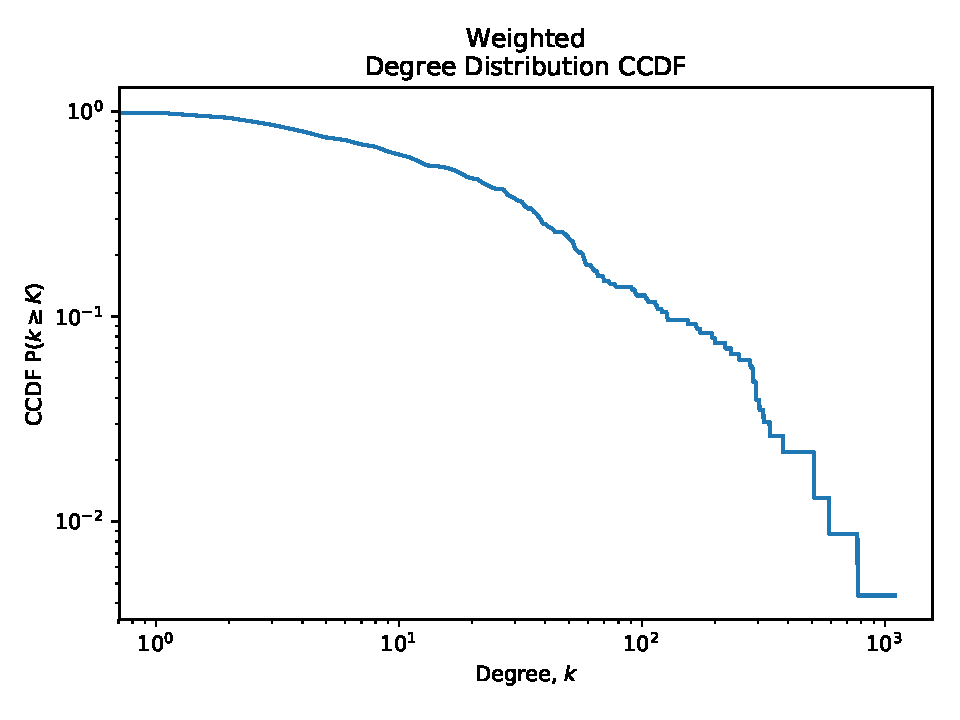
\includegraphics[width=1.\textwidth]{images/weighted_degree_distr_ccdf.pdf}
        \caption{Weighted degree distribution.}
    \end{subfigure}
    \begin{subfigure}{0.4\textwidth}
        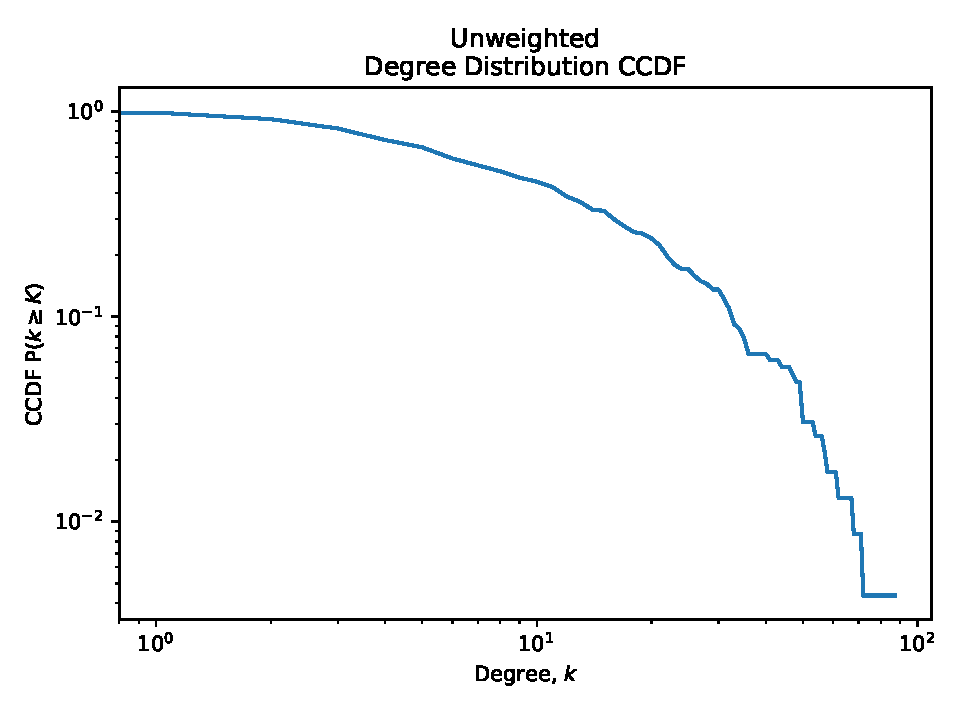
\includegraphics[width=1.\textwidth]{images/unweighted_degree_distr_ccdf.pdf}
        \caption{Unweighted degree distribution.}
    \end{subfigure}
    \caption{Degree distributions on a log-log scale. The distribution has a heavy tail, but does not follow a power law.}
    \label{fig:degree_distr}
\end{figure}

The degree distributions for the weighted and unweighted networks are shown as a CCDF in Figure~\ref{fig:degree_distr}. We see a heavy tail like we as expect from many real-world networks, but neither the unweighted nor the weighted degree distribution show a power law in the tail. 

Particularly in the unweighted network, the degree distribution has more high-degree nodes than would expected if the network were a Poisson random graph, though the tail drops of more quickly than expected in a scale-free network.

The weighted degree distribution has a heavier tail than the unweighted one, suggesting the distribution of character mentions is more uneven than the distribution of character interactions. The weighted network is closer to a power law, but not close enough to call scale-free.

We only speculate on the attachment mechanism behind the degree distribution. Vertex copying and preferential attachment do not make sense, as the degree distribution does not follow a power law. However, it seems reasonable that main characters receive more attention in a narrative network than would be expected in other kinds of networks, explaining some of the heavy tail.

The average unweighted degree is $13.31$ and the average weighted degree is $55.95$.

\subsection{Clustering}
We examine the fraction of closed triads by applying the transitivity definition of the clustering coefficient:

$$ C = \frac{\text{(number of triangles)} \cdot 3}{\text{number of connected triples}} $$

This metric disregards edge weights and looks at only the connections between characters. We find $C = 0.3930$, reflecting a fairly high density of connections -- likely a result of the strong community structure in Enfield Tennis Academy and the Halfway House. We do \textit{not} observe a tree-like structure rooted at the highest-degree (main) characters.

To determine if this effect is due to the degree sequence alone or reflective of author choice, we compare the book's clustering coefficient to an estimate produced by the averaging 100 configuration model simulations. Our simulations produce an average local clustering coefficient of 0$.1728$ -- significantly lower than what was found in the book's network.

We also compare the clustering coefficient against 5 of the smallest networks in the FB100 dataset. These networks range in size from $n=769$ to $n=1659$, significantly larger than the network present in \infinitejest. We find an average clustering coefficient of $0.2403$, which is closer to the book's results than our configuration model simulations. It seems that the book's network is more clustered than a real-world social network. It's worth noting that Alberich et al.\ (2002) found their Marvel network was \textit{less} clustered than real-world social networks.\cite{2002marvel}

\subsection{Modularity}
The book's characters generally fall into one of two communities: Enfield Tennis Academy, or the Ennet House. We label these and a few other, smaller communities: the Wheelchair Assassins, the Antitois brothers, and persons associated with the US/ONAN government. The modularity of these hand-labeled communities is 0.291, calculated according to the following equation:

$$Q = \frac{1}{2m}\sum_{ij} \left(A_{ij} - \frac{k_ik_j}{2m} \right) \delta(c_i,c_j) = \sum_u e_{uu} - a_u $$

A greedy modularity maximization algorithm successfully recovers these communities, though it does place high-degree nodes like Hal in their own community. Still, the greedy algorithm generates communities that are in high agreement with our hand-labeled set -- the two partitions have a Normalized Mutual Information of 0.605.

\begin{figure}[ht]
    \centering
    \begin{subfigure}{0.4\textwidth}
        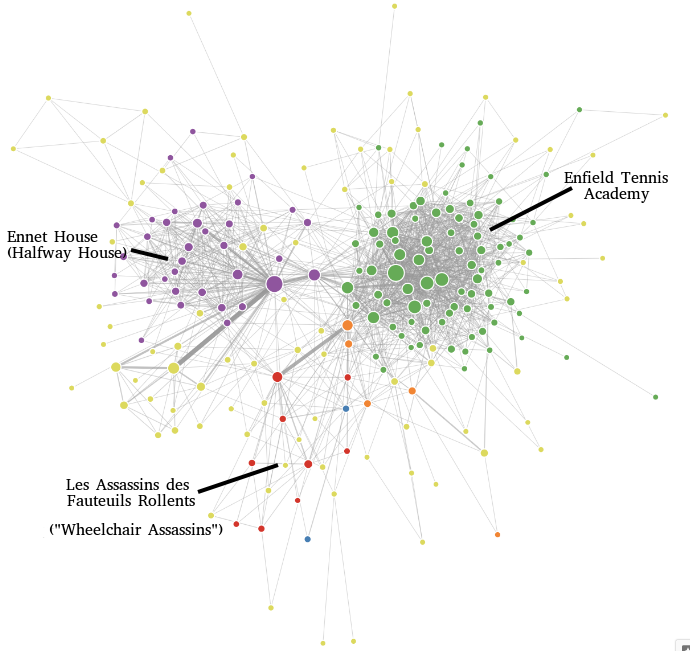
\includegraphics[width=1.\textwidth]{images/labeled_community_with_labels.png}
        \caption{Hand-labeled communities.}
    \end{subfigure}
    \begin{subfigure}{0.4\textwidth}
        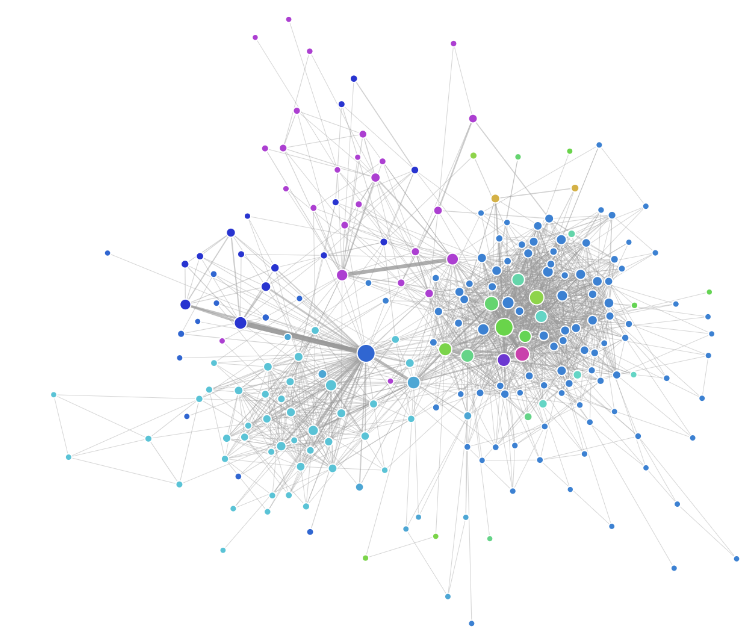
\includegraphics[width=1.\textwidth]{images/greedy_community.png}
        \caption{Communities detected by greedy modularity maximization.}
    \end{subfigure}
    \caption{The agglomerative greedy approach to modularity maximization recovered the hand-labeled communities.}
    \label{fig:modularity}
\end{figure}

The labeled communities and detected communities are visible in Figure \ref{fig:modularity}.

\subsection{Assortativity}
How do characters interact based on their association and gender?

\subsubsection{Degree Assortativity}
We observe an unweighted degree assortative mixing coefficient of -0.0945, showing some degree disassortativity. Degree assortative networks typically reflect core-periphery structures, where a dense core of highly-connected nodes is surrounded by successively less-dense periphery nodes. Degree disassortative networks, on the other hand, are more often configured like a star, where high-degree nodes connected to low-degree. 

According to Newman in {\em Networks}, social networks are unusual in that they typically have a positive degree assortativity \cite{NewmanBook}. Therefore it is strange for us to see disassortative mixing by degree in \infinitejest. This indicates either a star-like structure or fewer community structures than would be expected of a real-world social network.

\subsubsection{Gender Assortativity}
To examine gender assortativity, we label the characters with a gender attribute where the gender was clear from the text. Of 229 nodes, 27 have no label assigned to them. We find the assortativity to be 0.0858, indicating positive assortative mixing by gender: genders of the same type are more likely to co-occur in this text. This is not particularly unexpected; as students who board at Enfield Tennis Academy do so separated by gender.

\subsection{Centralities} 

Who are the most important characters in the \infinitejest? There are, of course, many ways to answer that question. The top eight characters under degree and betweenness centralities can be found in Table \ref{tab:centralities}.

\begin{table}[]
\begin{tabular}{@{}lllll@{}}
\toprule
 & \multicolumn{4}{c}{\textbf{Centralities}} \\ \midrule
 & \multicolumn{2}{l}{\textbf{Degree}}  & \multicolumn{2}{l}{\textbf{Betweenness}} \\ \midrule
\textbf{1} & Hal Incandenza   & 0.382 & Donald Gately   & 0.259 \\ \midrule
\textbf{2} & Donald Gately    & 0.311 & Hal Incandenza  & 0.140 \\ \midrule
\textbf{3} & Avril Incandenza & 0.294 & Joelle Van Dyne & 0.079 \\ \midrule
\textbf{4} & Aubrey DeLint    & 0.268 & Charles Tavis   & 0.065 \\ \midrule
\textbf{5} & Gerhardt Schtitt & 0.250 & Remy Marathe    & 0.056 \\ \midrule
\textbf{6} & Michael Pemulis  & 0.246 & John Wayne       & 0.051 \\ \midrule
\textbf{7} & Charles Tavis    & 0.232 & Gerhardt Schtitt & 0.049 \\ \midrule
\textbf{8} & James Incandenza & 0.215 & Michael Pemulis  & 0.048 \\ \toprule
\end{tabular}
    \caption{Top degree and betweenness centralities.}
    \label{tab:centralities}

\end{table}

\subsubsection{Degree Centrality}

We use degree centrality -- a proxy for mentions in our network structure -- to identify the characters with the most narrative space devoted to them and find it is able to recover the characters expected. It does tend towards characters associated with Enfield Tennis Academy, however.

\subsubsection{Betweenneness Centrality}
We use betweenness centrality to determine the characters who are most important in connecting the novel's far-flung threads. Donald Gately and Joelle van Dyne, the characters ranked highest by this measure other than Hal, are the only characters with significant connections to both Enfield Tennis Academy and Ennet House. Don also has interactions with the Wheelchair Assassins.

\subsection{Gender}

\infinitejest has received significant criticism for its treatment of women.\cite{hayes-brady_2017} We explore the question of bias in the book quantitatively. We find $144$ male entities, $58$ female entities, and $27$ entities of indeterminate or unknown gender; there are nearly two-and-a-half times as many men as women.

\subsubsection{Average Degree by Gender}
Figure~\ref{average-node-degree-by-gender} shows the difference in average degree by gender. Average unweighted degree can be seen as a rough approximation for the expected connectedness of a character. Average weighted degree can be seen as a rough approximation of the expected strength of a character's relationships. There is a difference between the average unweighted degrees of men and women, but it is far less striking than the difference between the averages of their weighted degrees. There are outliers, but women tend clearly to appear less frequently.

\begin{figure}[ht!]
    \centering
    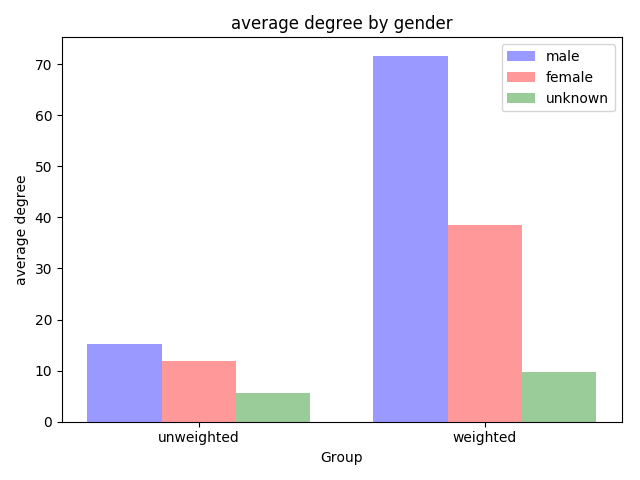
\includegraphics[width=.4 \textwidth]{images/gender_degrees.png}
    \caption{weighted and unweighted average node degree by gender}
    \label{average-node-degree-by-gender}
\end{figure}

\subsubsection{Degree Sequence Distribution by Gender}

Fgure~\ref{fig:degree_distr_gender} shows the weighted and unweighted degree distributions in CCDF, separated by gender. We see that, particularly in the weighted degree distribution, the plot for women has a significantly lighter tail than Figure~\ref{fig:degree_distr} might lead us to expect. This indicates there are a relatively large number of women with low degree, and there are some with high degree, but few in between.

\begin{figure}[ht]
    \centering
    \begin{subfigure}{0.4\textwidth}
        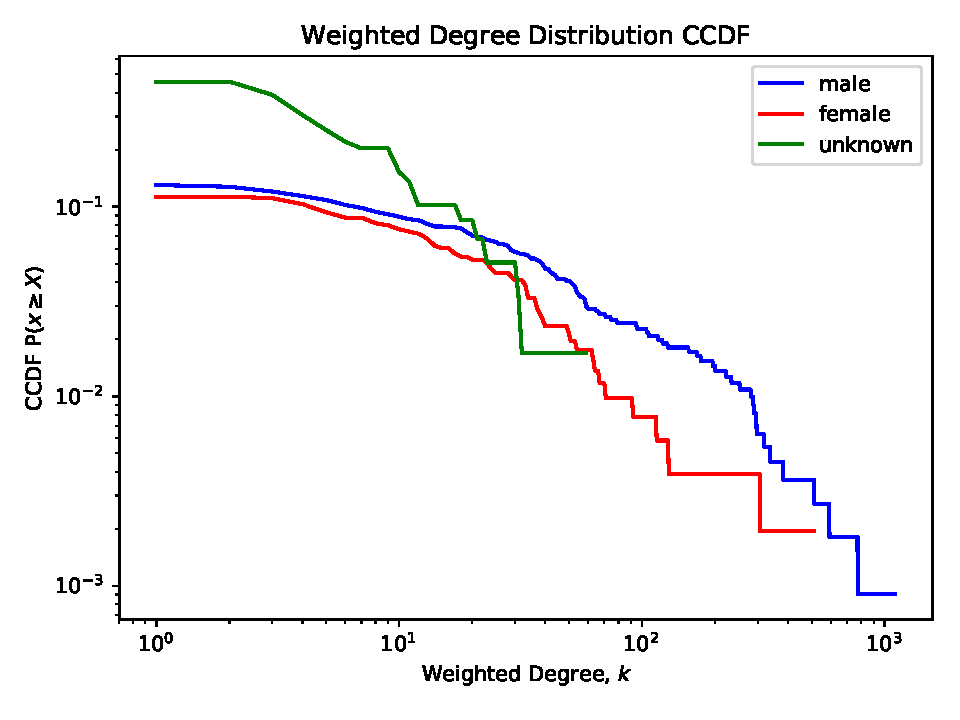
\includegraphics[width=1.\textwidth]{images/degree_distr_ccdf_gender_weighted-Weighted.pdf}
        \caption{Weighted degree distribution by gender}
    \end{subfigure}
    \begin{subfigure}{0.4\textwidth}
        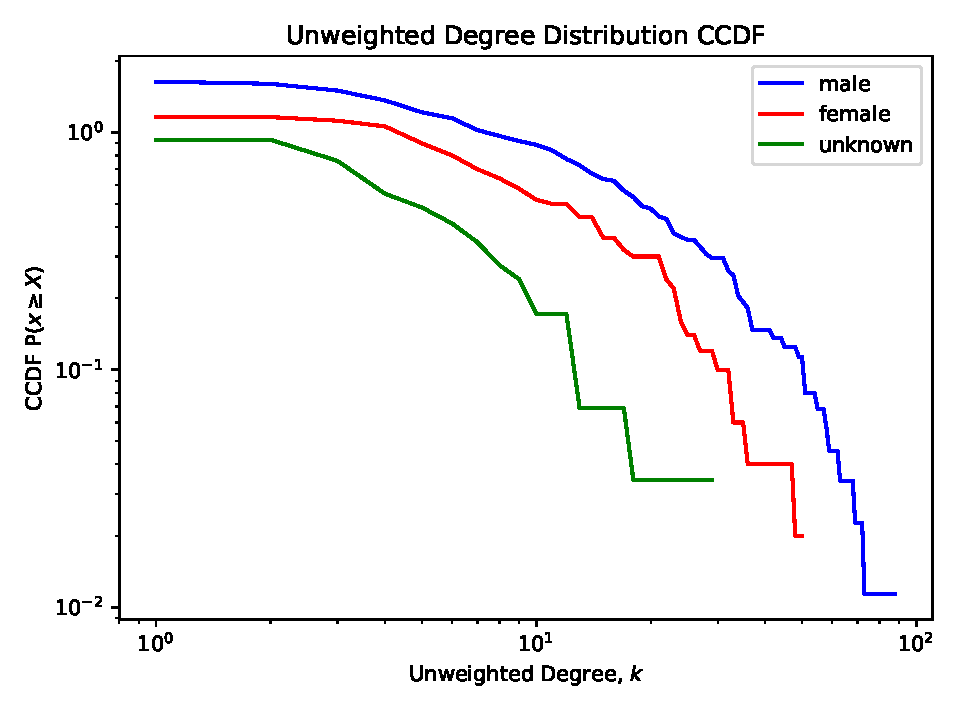
\includegraphics[width=1.\textwidth]{images/degree_distr_ccdf_gender_weighted-Unweighted.pdf}
        \caption{Unweighted degree distribution by gender}
    \end{subfigure}
    \caption{Degree distributions by gender on a log-log scale.}
    \label{fig:degree_distr_gender}
\end{figure}

\subsubsection{Betweenness by Gender}
To explore gender bias in character betweennesses, we run 100 simulations of a configuration model using the book's degree sequence to get an average of betweenness for each character. Figure~\ref{difference-in-betweenness} plots a histogram of the differences between the book's betweennesses and our estimates. It shows that, independent of gender, most characters have a significantly lower betweenness in the book than the simulations would lead us to expect, but that several characters in the book have \textit{wildly} higher betweennesses. It is worth noting that no characters with an indeterminate or unknown gender had a significantly higher betweenness than expected by the configuration model.

We find there are several male and female characters who have a priviliged position in the network. Unsurprisingly, these privileged characters are all important: Donald Gately, Joelle van Dyne, Avril Incandenza, and Hal Incandenza are among them. A high betweenness seems a reasonable consequence of narrative attention.
   
\begin{figure}[ht!]
    \centering
    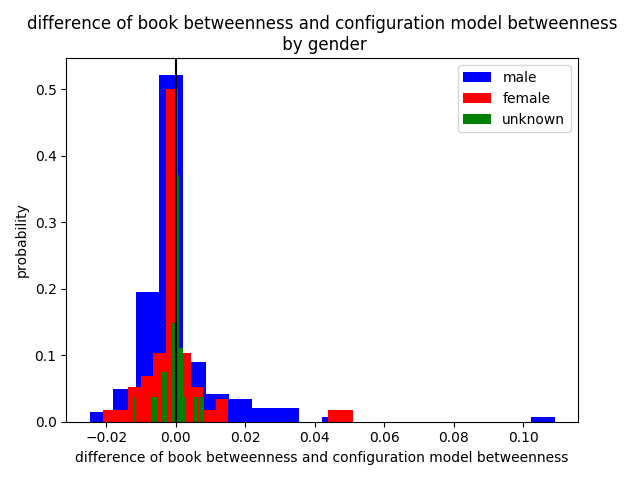
\includegraphics[width=.4 \textwidth]{images/gender_betweenness_by_gender.png}
    \caption{difference in book's betweennesses and those expected under the configuration model, by gender}
    \label{difference-in-betweenness}
\end{figure}
